\chapter{O banquinho}
\label{chap:banquinho}

Nos primórdios da humanidade, os seres humanos sentavam-se em
pedras, troncos de árvore, ou até mesmo montinhos de terra.
Com o passar do tempo, o ser humano passou a ser mais civilizado
e passou a fabricar ferramentas que o ajudassem no dia-a-dia.

Para sentar, o ser humano inventou um dispositivo revolucionário
chamado o \emph{banquinho} (vide Figura \ref{fig:banquinho}).

\begin{figure}[!htb]
  \centering
  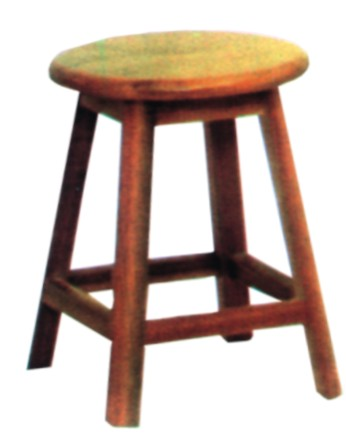
\includegraphics[width=0.5\textwidth]{banquinho.jpg}
  \caption{O banquinho}
  \label{fig:banquinho}
\end{figure}

%http://br.answers.yahoo.com/question/index?qid=20091125150826AA7YDiN
De acordo com fontes confiáveis (a segunda resposta de uma pergunta
no \textit{Yahoo! Answers}), o tamanho ideal de um banquinho hoje em
dia é de 60 a 70~cm.
